\pagestyle{empty}
\section{System Overview\\{\small\tt J.~Mitchard}}
\label{system_overview}
\subsection{Supervisor-Child Architecture}
\label{otp_description}
% another intro to OTP
% what is a SupervisorSupervisor-Child Architecture
% why this is useful
    % gen-servery stuff
The \verb+swarmer+ application has been implemented in a hierarchical process structure using Erlang Supervisor processes\footnote{http://www.erlang.org/doc/man/supervisor.html} that comes as part of the OTP\footnote{http://www.erlang.org/doc/design\_principles/des\_princ.html} \footnote{http://learnyousomeerlang.com/what-is-otp} (Open Telecom Platform). This means that all processes are children of a supervisor process within the applications' supervision tree. Supervisors are responsible for the stopping, starting and restarting of their child processes.
%
\label{supervisor_arch}
The \verb+swarmer+ application has been implemented in a hierarchical process structure using Erlang Supervisor processes\footnote{http://www.erlang.org/doc/man/supervisor.html}, a behaviour that comes as part of the OTP\footnote{http://www.erlang.org/doc/design\_principles/des\_princ.html} \footnote{http://learnyousomeerlang.com/what-is-otp} (Open Telecom Platform). This means that all processes are children of a supervisor process within the applications' supervision tree. Supervisors are responsible for the stopping, starting and restarting of their child processes.
\verb+Swarmer+ has one main supervisor, called the \verb+swarm_sup+, this is responsible for the \verb+tile_sup+, \verb+viewer_sup+, \verb+human_sup+, \verb+zombie_sup+, \verb+supplies_sup+ supervisor processes and the \verb+environment+ process.

Apart from \verb+swarm_sup+, all of the supervisors are created with a \verb+simple-one-for-one+ restart strategy, meaning that each of the children will be identical processes using the same code, and should be researted if they crash. \verb+swarm_sup+ is using a \verb+one-for-one+ strategy, which can restart it's child processes without affecting the others\footnote{http://www.erlang.org/doc/design\_principles/sup\_princ.html\#id68643}.

\begin{figure}[h]
  \centering
  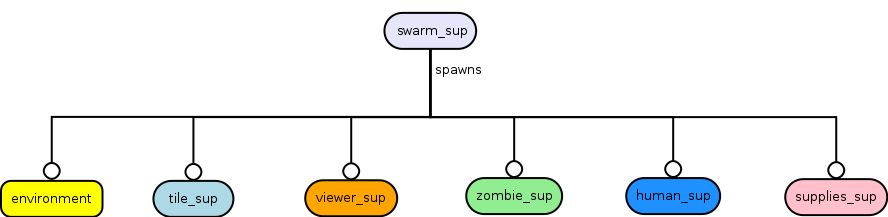
\includegraphics[width=0.8\textwidth]{img/supervisor.png}
\caption{Supervision Tree for Swarmer}
    \label{fig:sup_tree}
\end{figure}

\subsubsection{OTP Behaviours}
\label{otp_behaviours}
Using an Erlang and OTP application with a process supervision architecture provides a standard set of interface functions, behaviours and more advanced error tracing and reporting functionality.

The backbone of \verb+swarmer+ is created using the \verb+gen_server+\footnote{http://www.erlang.org/doc/design\_principles/gen\_server\_concepts.html} (Generic Server) behaviour. \verb+gen_server+ provides a framework for reliable and robust message passing between processes, using either synchronous requests called calls, or asynchronous request called a casts. The \verb+environment+, \verb+tile+, \verb+viewer+ and \verb+supplies+ modules have been implemented with \verb+gen_server+ behaviours.

The behaviour of the human and zombie entities in the system is modelled around the \verb+gen_fsm+\footnote{http://www.erlang.org/doc/design\_principles/fsm.html} (Generic Finite State Machine) behaviour. \verb+gen_fsm+ provides a state machine for the entities to use, and incorporates synchronisation events, such as pause and unpause, for the rest of the system to call. The \verb+gen_fsm+ processes will, once started, run until told to stop. The \verb+human_fsm+ and \verb+zombie_fsm+ modules have been implemented with \verb+gen_fsm+ behaviours.

\subsection{System Architecture}
\label{sys_overview_architecture}
As introduced in section \ref{supervisor_arch} \verb+swarmer+ is built around a Supervisor-Child architecture. This section will explain the setup of the application in a little more detail.

When the application is started, the initial process is an instance of the \verb+swarm_server+ module. This is responsible for starting the Websocket and spawning the system supervisor module, \verb+swarm_sup+. The system uses the Cowboy\footnote{http://ninenines.eu/docs/en/cowboy/1.0/guide} HTTP server to manage Websocket communication to the user client, which is covered in section \ref{client_doc}. The web socket is managed by a module called \verb+swarm_handler+.

\begin{figure}[h]
  \centering
  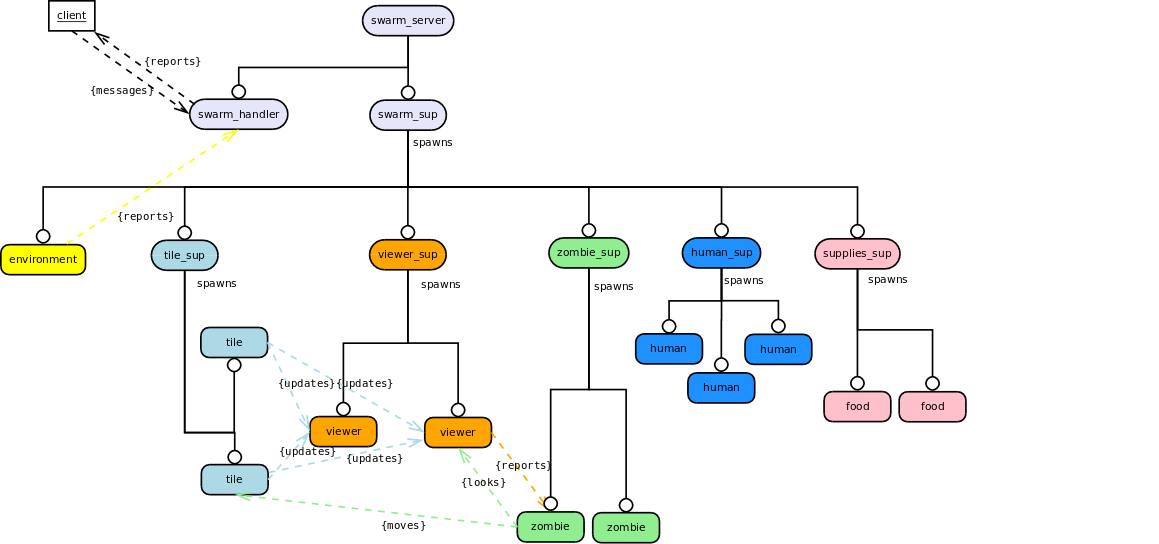
\includegraphics[width=0.8\textwidth]{img/final_system_ws.png}
\caption{System Architecture}
    \label{fig:system_ws}
\end{figure}

On initialisation, the \verb+swarm_sup+ will spawn the children processes shown in figure \ref{fig:sup_tree} and the system will wait for a message from the client to define what to spawn, this will be covered in section \ref{system_setup}. Once received, it will then continue waiting until \verb+swarm_handler+ receives a message to start the system.

In order to visualise what is happening in the system, the client systematically requests a report from \verb+swarmer+. To report back to the client, the \verb+environment+ module requests the status of all of the supervisors children nodes. This is returned to \verb+swarm_handler+ which is encoded into a JSON object using the \verb+jsx+ dependency and sent to the client.

\begin{figure}[h]
  \centering
  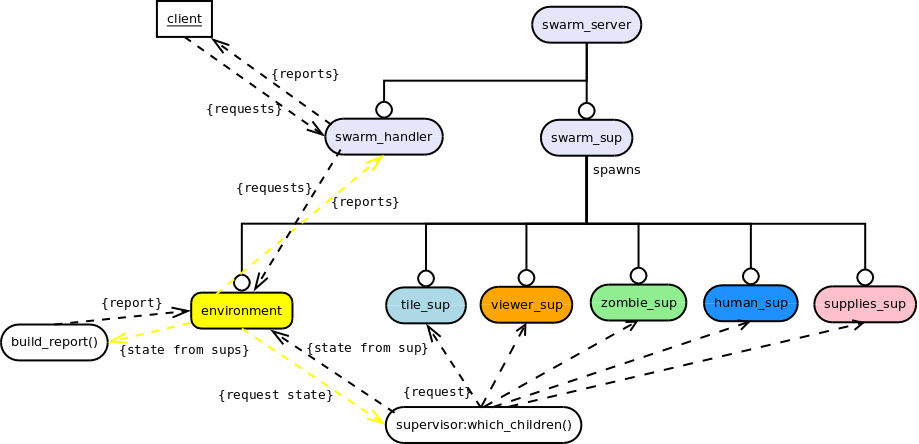
\includegraphics[width=0.8\textwidth]{img/client_report.png}
\caption{Reporting to the Client}
    \label{fig:client_report}
\end{figure}

The map is created out of a grid of \verb+tile+ instances with assigned \verb+viewer+ instances. This is explained in more detail in section \ref{tiles_and_viewers}. When the entities are initially spawned they are initialised in a paused state until the system is told to start. After this, the entities begin to run carrying out their type specific behaviours. The way in which entities interact with the environment is explained in detail in section \ref{entities_awareness}. Zombies, covered in section \ref{zombie_doc}, in the simulation are created as an instance of the \verb+zombie_fsm+ module, and attempt to find human entities in the environment. Over time they will slow down if they have not eaten in a long time, and can turn human processes into zombies if they succeed in killing one, thus spreading the swarm. Humans on the other hand are trying to survive, meaning they must scavenge for food and escape the horde of zombies. Their behaviour is covered in section \ref{human_doc}.

\subsection{System Setup}
\label{system_setup}
The initial set-up of the simulation environment is handled by the \verb+environment+ module. This deals with spawning \verb+tile+, \verb+viewer+, \verb+supplies+, \verb+human_fsm+ and \verb+zombie_fsm+ processes according to the set-up instructions received from \verb+swarm_handler+. On a normal set-up, the system would be told to create an amount of tiles, defined by a 'grid arrity' and an amount of each entity type to spawn. Grid arrity would be an integer between the value of 1 and 10, 1 telling the system to build a 1x1 grid and 10 telling the system to build a 10x10 grid.

Obstructions, which are covered in section \ref{los}, play a big part in the way our simulation runs, they block line of sight and prevent movement through them. During the initial setup, this is created through a list of blocked coordinates passed into the tiles on initial set-up.

\subsubsection{Making the Grid}
When the \verb+environment+ process receives a \verb+make_grid+ request it will firstly purge the system of currently spawned processes; restarting the system from the ground up. This prevents old instances of processes remaining in the supervision tree.

The process will then proceed to create a grid of given arrity by spawning \verb+tile+ instances of a given size. In order to create a grid like structure, a row of tiles is spawned, assigning each an origin coordinate and an end coordinate before creating another row of tiles. All \verb+tile+ processes are registered to Erlang as a named process of the form "tileXOYO", O being the origin point for each axis. Each of these is then has a viewer process assigned to it.

\clearpage
\endinput
